\documentclass[11pt,a4paper]{jreport}

\usepackage{authblk}
\usepackage{algorithm}
\usepackage[noend]{algpseudocode}
\usepackage[dvipdfmx]{graphicx}
\usepackage{mathptmx}
\renewcommand\Authsep{\qquad}
\renewcommand\Authand{\qquad}
\renewcommand\Authands{\qquad}

%%%%%%%%%
% 講究録用(著者情報)
\author[1]{佐藤明幸}
\author[2]{山本博章}
\author[3]{藤原洋志}

\affil[1]{
 信州大学大学院総合理工学研究科 \authorcr
 Graduate School of Science and Technology, Shinshu University
}
\affil[2]{
 信州大学大学院総合理工学研究科 \authorcr
 Graduate School of Science and Technology, Shinshu University
}
\affil[3]{
 信州大学大学院総合理工学研究科 \authorcr
 Graduate School of Science and Technology, Shinshu University
}
% end of 講究録用
%%%%%%%%%

\setlength{\topmargin}{-0.3cm}
\setlength{\textheight}{23cm}
\setlength{\oddsidemargin}{0.5cm}
\setlength{\textwidth}{15.0cm}

\date{}

\begin{document}
  \begin{titlepage}
      \begin{center}
          \vspace*{180truept}

          {\Huge ファクターオラクルを用いたコンパクトな全文検索索引の構築.} 

          \vspace{200truept}

          {\Large 2021年1月31日}

          \vspace{30truept}

          {\Large 佐藤 明幸}      

      \end{center}
  \end{titlepage}


  \chapter{序論}
  \section{研究の背景}
 全文検索問題とは、文字列集合$D = T_0 .. T_n$から検索したいパターン$p$の(テキスト番号, 維持番号)の組からなる位置情報をすべて出力する問題である。簡潔に述べると、複数のテキストファイルから特定のパターンの出現位置を探すということである。
 
 情報処理の多くの分野において全文検索問題を含むパターンマッチングの問題は重要な問題であり、データ処理、文書編集、字句解析、情報検索の中でよく使われる。ウイルス対策ソフトがウイルスを発見するための最も一般的な方式として用いられる。また、多くのテキストエディタやプログラミング言語にはパターンを照合する機能が含まれている。この問題は情報工学において中心的な問題として幅広く研究されたものの一つである。

 全文検索問題へのアプローチとしては大きく分けて逐次型と索引型に分類される。逐次型は検索対象となる複数のファイルをそれぞれ逐次に探索し、検索パターンを全て探し出すため、検索にテキスト長に比例した時間がかかってしまう問題がある。これに対し索引型では、事前にテキストから作成した索引を検索に用いることで検索を高速化することができる。ただし索引の作成には時間がかかり、検索を行うためには索引を保持するためのメモリ空間が必要となることに留意しなければならない。一般的な索引型の手法としてはSuffix array等のデータ構造を用いたものがある。他にはDAWG(Directed Acyclic Word Graph)\cite{dawg}というオートマトンを使用した手法があり、こちらはビット列で表現することでSuffix arrayを使用した場合よりも少サイズとなることが\cite{dawg-bit}で述べられていた。

 Allauzen 他は、文字列に対し、ファクターオラクルと呼ばれる新たなデータ構造を考案し、文字列パターン照合に応用した。文字列$w$に対するファクターオラクル\cite{allauzen}は、少なくとも$w$のすべての部分文字列を受理するオートマトンである。状態数は$|w|+1$、遷移数は$2|w|-1$である。

 ファクターオラクルを索引に用いる難しさは、あるテキスト$w$から構成されたファクターオラクル$Oracle(w)$があるパターン$p$を受理したとき、もとのテキスト$w$に$p$が出現しているかどうかわからない擬陽性をもつという点にある。

 ファクターオラクルを用いることでほぼ線形時間でパターンマッチングを行うアルゴリズム\cite{kato}が知られている。

 ファクターオラクルが単一の文字列から構成されるのに対し、先行研究\cite{ohi}では、複数文字列に対するファクターオラクルを定義することで、全文検索索引へ活用していた。また、DAWGを用いた場合よりも状態数、遷移数共に少サイズで表現できることが実験的に述べられていた。

  \section{研究の目的}
  単一のテキストに対する効率的な検索手法は数多く提案されてきたが、複数の文字列集合の対する全文検索の手法は多くはない。

 そこで先行研究では、文字列集合からトライ木を構成し、そのトライ木を入力としてファクターオラクルと部分集合木を構成し全文検索索引としていた。しかしこの方法では構成、検索の共に線形時間で実行することは不可能であった。

 本研究では、先行研究の問題を解決し、ファクターオラクルを用いた線形時間で構築と検索が可能な全文検索索引を提案することを目的とする。

  \chapter{諸定義}

  \section{オートマトン}
  一般的にオートマトンとは、入力によって内部状態を遷移させ、処理や入力を行う計算機モデルである。図にあるような状態遷移図として表される。

  \begin{figure}[htbp]
    \centering
    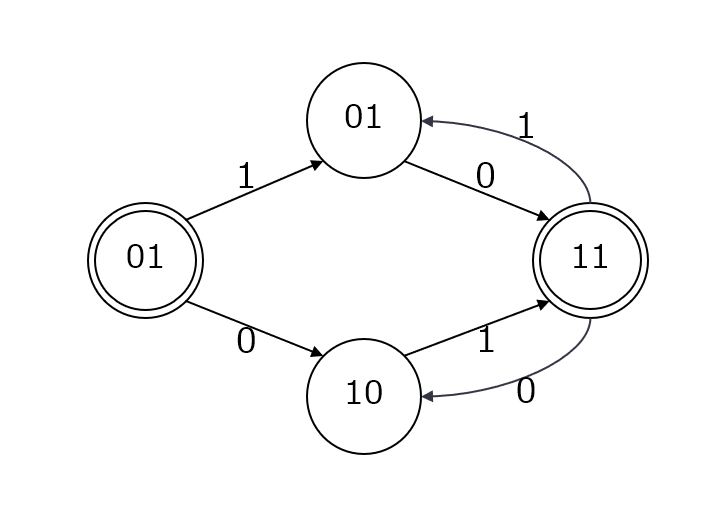
\includegraphics[width=10cm]{automaton.png}

    \caption{オートマトン例図}
  \end{figure}

  図中の丸が状態を表しており、矢印が外部からの入力によってどの状態に映るかを表している。ここで、初期状態は状態00であり、1を入力とした場合には状態01へ、0を入力とした場合には状態10へ状態を遷移することになる。さらに、二重丸で表された状態のことを特に受理状態という。全ての入力を受け、遷移し終わった後に、受理状態に到達した場合、オートマトンが入力を受理したことになり、受理と出力する。そうでない場合は非受理となる。
  状態と入力によって次に遷移する状態が一位に定まり、状態数が有限このものを決定性有限オートマトン(DFA)という。図の例では空気号列か、松木が10または01で終わる文字列を受理する決定性有限オートマトンである。

  決定性有限オートマトン$M$は以下の5字組で定義される。
  $$
    M = (Q, \Sigma, \delta, q_0, F)
  $$
  ここで、\\
  $Q: 状態(state)の有限集合$\\
  $\Sigma: 入力記号(input symbol)の有限集合$\\
  $\delta: 遷移関数(move function) (\delta: Q \times \Sigma \rightarrow Q)$\\
  $q_0: 初期状態$\\
  $F: 受理状態の有限集合$\\である。

  \section{全文検索問題}
  任意の文字列$w, x, y, z \in \Sigma^*$に対し、$w = xyz$と表すことができるとき、$xをw$の\textbf{接頭辞}、$zをw$の\textbf{接尾辞}, $yをw$の\textbf{部分文字列}と呼ぶ。このとき、$FACT(w)$を$$FACT(w) = \{ y\,|\,yはwの部分文字列\}$$と定義する。

  検索対象となる文字列を\textbf{テキスト}といい、$T$と表す。また、検索する文字列を\textbf{パターン}といい、$P$と表す。テキストには先頭の文字から1文字ずつ順に番号を付ける。これを\textbf{位置番号}と呼ぶ。$n$文字あるテキスト$T$は$T=t_1t_2...t_n$と表す。テキストがN個ある場合、文字列集合を$D$とおき、$D={T_1, T_2,..., T_N}$と表す。議論の簡単化のため、$任意のT_iはいかなるT_j$の接頭辞ではないとする。各テキストにつけられた番号を\textbf{文章番号}と呼ぶ。本研究における全文検索問題とは、$P$が与えられたとき、$P \in FACT(D)$を満たす文章を見つけ、その文章番号と位置番号の組を全て出力する問題である。

  $L(M)をDFA M$によって受理される言語とすると、$$FACT(D) = \{y\,|\,\exists w \in L(M), yはwの部分文字列\}$$と定義する。このことより、本研究では$FACT(D)$に含まれる全ての部分文字列を受理できるオートマトンを構成し、そのオートマトンに入力として文字列$P$を与え、受理可否受理であるかを見ることで全文検索を実現する。

  \chapter{ファクターオラクル}
  \section{ファクターオラクルとは}
 ファクターオラクル\cite{allauzen}はAllauzen他によって1999年に発表されたオートマトンである。$p$に対するファクターオラクル$Oracle(p)$は、以下の性質を持つ。
  \begin{enumerate}
    \item 少なくとも$p$のすべての部分文字列を受理する。
    \item 全ての状態が受理状態である。
%    \item 閉路を持たない決定性有限オートマトンである。
    \item 状態数が$|p|+1$個、遷移数が$2|p|-1$個以下
    \item 受理した文字列が入力のテキスト$p$に含まれていない可能性がある。すなわち$Oracle(p)$は\textbf{擬陽性}を持つ。
  \end{enumerate}

  \section{Allauzenの構成アルゴリズム}
  本章では、ファクターオラクル$Oracle(p)$の構成法を示す。ここで、アルゴリズムで使用するsupply function\ $S$を以下のように定義する。

  \begin{figure}[htbp]
    \centering
    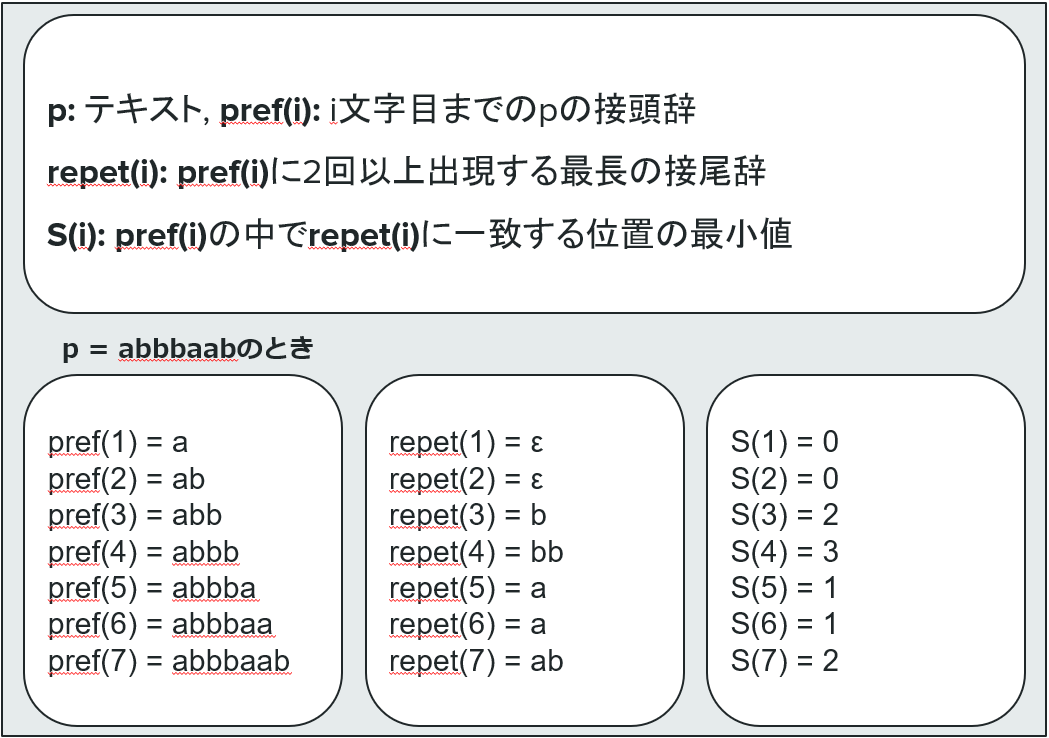
\includegraphics[width=12cm]{defsup.png}
    \caption{supply function\ $S$の定義}
  \end{figure}
  \newpage

  ファクターオラクルは以下のあるテキスト$p$を引数としてオンラインアルゴリズムcreate\_oracleで構成される。
  \begin{algorithm}
    \caption{$\textbf{create\_oracle}(p=p_1p_2...p_m)$}
    \label{alg1}
    \begin{algorithmic}[1]
      \State $Create\ Oracle(\epsilon)\ with:$
      \State $\ \ \ \ one\ single\ state\ 0$
      \State $\ \ \ \ S_\epsilon(0) \leftarrow -1$
      \For{$i \leftarrow 1..m$}
      \State $Oracle(p_1p_2...p_i) \leftarrow add\_letter(Oracle(p=p_1p_2...p_{i-1}), p_i)$
      \EndFor
    \end{algorithmic}
  \end{algorithm}
  
  create\_oracleはオンラインアルゴリズムであり、テキスト$p$を1文字ずつ読み込み内部で関数add\_letterを呼び出している。関数add\_letterの定義は以下のようになっている。

  \begin{algorithm}
    \caption{$\textbf{add\_letter}(Oracle(p=p_1p_2...p_m), \sigma)$}
    \label{alg2}
    \begin{algorithmic}[1]
      \State $Create\ a\ new\ state\ m+1$
      \State $Create\ a\ new\ transition\ from\ m\ to\ m+1\ labbeled\ by\ \sigma$
      \State $k \leftarrow S_p(m)$
      \While{$k>-1\ and\ there\ is\ no\ transition\ from\ k\ by\ \sigma$}
      \State $Create\ a\ new\ transition\ from\ k\ to\ m+1\ by\ \sigma$
      \State $k \leftarrow S_p(k)$
      \EndWhile
      \If{$k=-1$}
      \State $s \leftarrow 0$
      \Else
      \State $s \leftarrow where\ leads\ the\ transition\ from\ k\ by\ \sigma.$
      \EndIf
      \State $S_{p\sigma}(m+1) \leftarrow s$
      \Return $Oracle(p=p_1p_2...p_{m\sigma})$
    \end{algorithmic}
  \end{algorithm}

  具体例として、$p=$'abbbaab'をcreate\_oracleの実行例を以下に示す。
  \newpage

  \begin{figure}[htbp]
    \centering
    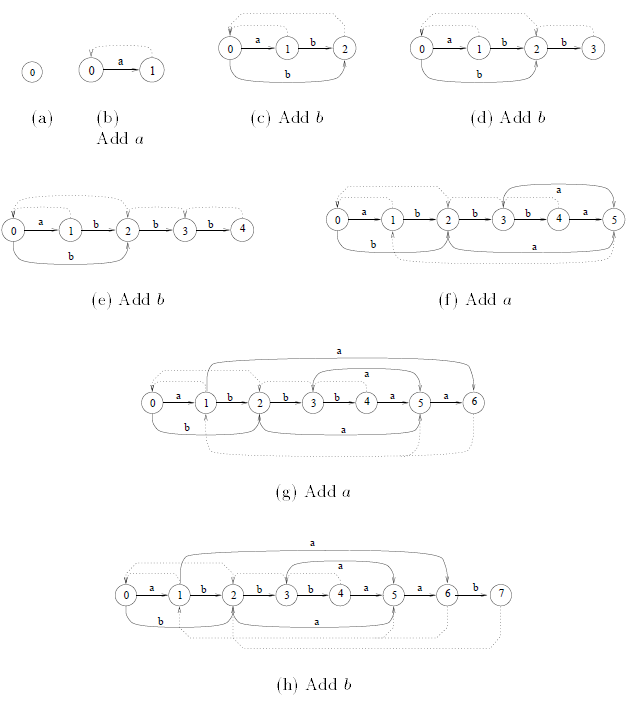
\includegraphics[width=14cm]{createfo.png}
    \caption{create\_oracleによるOracle('abbbaab')の構成例\ 点線はsupply functionを示す\ \cite{allauzen}より引用}
  \end{figure}

  \subsection{内部遷移}
  アルゴリズム2の2行目で作られた遷移を内部遷移と定義する。

  内部遷移をたどることで入力のテキストを保持することなく参照することができ、索引が使用するメモリの量を削減することができる。

  \newpage
  \section{サフィックスリンクツリー}
  前節で述べたように、ファクターオラクルは状態数と遷移数が少なく、効率的なオートマトンであるが、擬陽性を持つ。Oracle('abbbaab')では、入力のテキスト'abbbaab'の部分文字列ではないパターン'aba'を誤って受理してしまうことが確認できる。

  ファクターオラクルを部分文字列検索の検索索引として使用するためにはこの擬陽性を解消する必要がある。\cite{kato}では、擬陽性を解消し、更に効率的に検索を行うためにサフィックスリンクツリーという木構造が定義されていた。  

  図3.2で点線で各状態をつないでいたsupply functionの値を全てつなげたものがサフィックスリンクツリーである。
  Oracle('abbbaab')に対するサフィックスリンクツリーを以下に示す。
  \begin{figure}[htbp]
    \centering
    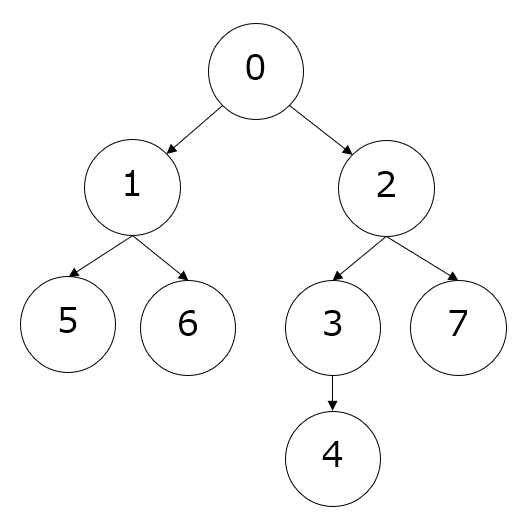
\includegraphics[width=8cm]{slt.png}
    \caption{Oracle('abbbaab')に対するサフィックスリンクツリー}
  \end{figure}

  \section{検索アルゴリズム}
  本節では、ファクターオラクルとサフィックスリンクツリーを用いた部分文字列検索アルゴリズムを紹介する。

  ここで、以下を定義する。
  \begin{enumerate}
    \item $S^{-1}(i)はOracle(p)のサフィックスリンクツリーのノードiの全子ノードの集合$
    \item $SP^{-1}(i)はOracle(p)のサフィックスリンクツリーのノードiの全子孫ノードの集合$
  \end{enumerate}

  \begin{algorithm}
    \caption{$\textbf{find\_all\_occurence}(Oracle(p), w)$}
    \label{alg3}
    \begin{algorithmic}[1]
      \If {$w\ recognized\ by\ Oracle(p)\ at state\ \overline{w}$}
      \State $i \leftarrow \overline{w}\ of\ Oracle(p)$
      \Else
      \Return $\emptyset \ \ \ \ \ \ \ \ \ \ \ \ \ \ \ \ \ /*\ empty\ set\ */$
      \EndIf
      \If {$p[(i-|w|+1)...i]=w$}
      \State $output\leftarrow i$
      \EndIf

      \For{$j \in S^{-1}(i)$}
      \If {$p[(j-|w|+1)...j]=w$}
      \State $output\leftarrow output \cup SP^{-1}(j)$
      \EndIf
      \State \textbf{else}\ $contiue$
      \EndFor
      \Return {$output$}
    \end{algorithmic}
  \end{algorithm}
  \newpage

  検索アルゴリズムは、
  \begin{enumerate}
    \item まず最初に入力のパターン$w$で$Oracle(p)$を遷移させ、受理した状態番号$\overline{w}$を得る。受理しなければ空集合を返す。
    \item その状態番号に対応するテキスト$p$の位置に$w$が出現していれば出現位置の集合$output$に$\overline{w}$を追加する。
    \item $Oracle(p)$があるパターン$w$を受理した場合の出現位置の候補は$\overline{w}$だけではなく、$SP(\overline{w})$の全てに及ぶ。よって、Algorithm\ 3の9行目からは、テキスト$p$の各$j \in S^{-1}(\overline{w})$の値に対して$w$が出現しているか判定している。もし出現していれば、$outputにSP^{-1}(j)$を追加し、そうでなければ追加しない。
  \end{enumerate}

  このアルゴリズムは、$\mathcal{O}(|S^{-1}(\overline{w}) \times w)$の実行時間を要す。$\mathcal{O}(|S^{-1}(i))|$は最悪で$\mathcal{O}(p)$になる。しかし、$Oracle(p)$のサフィックスリンクツリーのノード数が$p$であるため、ならし計算量では$\mathcal{O}(1)$となることがわかる。

  よってアルゴリズム全体でのならし計算量は$\mathcal{O}(w)$である。

  \chapter{文字列集合に対するファクターオラクル}
  前章では、単一のテキストに対して効率的に検索を可能にするデータ構造を紹介した。我々の研究では複数のテキストを含むような文字列集合に対して、効率的に検索を行いたい。本章では、先行研究\cite{ohi}で提案されていた文字列集合に対するファクターオラクルを用いた全文検索索引について解説する。

  \section{文字列集合に対するファクターオラクルとは}
  文字列集合に対するファクターオラクルは、ファクターオラクルを全文検索に応用するために\cite{ohi}で定義されている。

  \section{構成アルゴリズム}
  文字列集合に対するファクターオラクルは、
  \begin{enumerate}
    \item 入力の文字列集合からトライ木を構成する
    \item トライ木に部分集合構成法を適用する
  \end{enumerate}
  以上の手順で構成される。

  \subsection{トライ木の構成}

  \begin{algorithm}
    \caption{$\textbf{BuildDFA}(D)$}
    \label{alg4}
    \begin{algorithmic}[1]
      \State Input $D={T_1,T_2,...,T_N}$
      \State $s \leftarrow 0,Q \leftarrow \{s\}, statenum \leftarrow 0$
      \For {$i=1...N$}
        \For {$j=1...N$}
          \If {$\delta(s,t_j=s')$}
          \State $s \leftarrow s'$
          \Else
          \State $statenum \leftarrow statenum+1$
          \State $\delta(s,t_j)=statenum,Q \leftarrow Q \cup \{statenum\}$
          \State $s \leftarrow statenum$
          \EndIf
        \EndFor
        \State $F \leftarrow F \cup \{s\}$
      \EndFor
      \Return $M = (Q, \Sigma, \delta, q_0, F)$
    \end{algorithmic}
  \end{algorithm}
  \newpage

  $BuildDFA$を$D=\{"abbac", "aaaac"\}$を入力として実行した例を以下に示す。

  \begin{figure}[htbp]
    \centering
    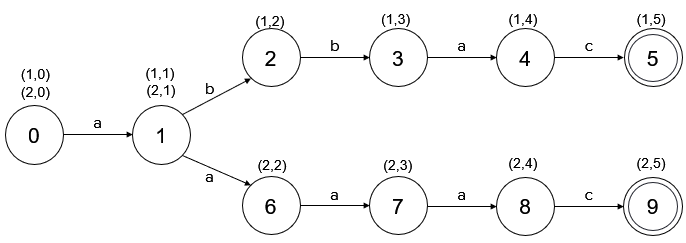
\includegraphics[width=15cm]{trie.png}
    \caption{$D=\{"abbac", "aaaac"\}$を入力としたときのトライ木}
  \end{figure}
  
  \subsection{文字列集合に対するファクターオラクルの構成}
  本説では文字列集合に対するファクターオラクルの構成法を示す。本アルゴリズムは前節で示したアルゴリズムで構成したトライ木の全ての状態を初期状態と置き、非決定性有限オートマトン(NFA)からDFAを構成する\textbf{部分集合構成法}を、応用したアルゴリズムである。また、$s=\{i_1,i_2,...,i_j\}(i_1<i_2<...<i_j)をトライ木$M$の状態の部分集合としたとき、min(s)=i_1$と定義する。%まず、前節で示したアルゴリズムで構成したトライ木を入力とする。トライ木の全ての状態の集合$Q$を初期状態$q_0$と置き、任意の部分集合$Q_1 \subset Q$と任意の入力記号$a \in \Sigma$に対して、$\delta(Q_1, a)=Q_2 \subset Q$を作成し、もしくはすでに存在していたらその状態に遷移する。本アルゴリズムでは追加条件として


  \begin{algorithm}
    \caption{$\textbf{BuildOracle}(M)$}
    \label{alg5}
    \begin{algorithmic}[1]
      \State Input $M = (Q, \Sigma, \delta, q_0, F)$
      \State $s_0 \leftarrow Q, m \leftarrow |Q|, Q' \leftarrow {s_0}$
      \For {$i=0...m$}
        \State $sをmin(s)=iになるQ'の状態とする。もしこのような状態がなければ\ next$
        \For {\textbf{all} $\sigma \in \Sigma$}
           \State $s'=\delta(s,\sigma)を計算する$
           \If {$minn(s')=min(t)となるtが存在する$}
           \State $\delta'(s,\sigma)=t$
           \Else
           \State $\delta'(s,\sigma)=s',Q'\leftarrow Q' \cup \{s'\}$
           \EndIf
        \EndFor
      \EndFor
      \State $F'=Q'$
      \State \textbf{return}\ $M_{FO} = (Q', \Sigma, \delta', q_0, F')$
    \end{algorithmic}
  \end{algorithm}

  $BuildOracle$を$D=\{"abcba", "abbac"\}$から構築したトライ木を入力として実行した例を以下に示す。

  \begin{figure}[htbp]
    \centering
    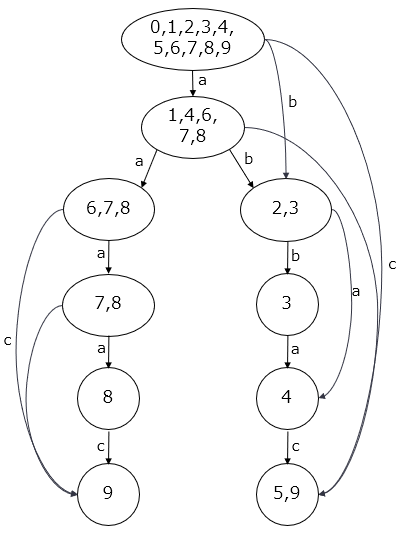
\includegraphics[width=10cm]{sub.png}
    \caption{$D=\{"abcba", "abbac"\}$から構築したトライ木を入力としたときの文字列集合に対するファクターオラクル}
  \end{figure}

  文字列集合に対するファクターオラクルは少なくとも$FACT(D)$の全ての文字列を受理するが、擬陽性を持つ。

  \section{全文検索アルゴリズム}
  本節では文字列集合に対するファクターオラクルを使用した全文検索アルゴリズムを示す。

  文字列集合に対するファクターオラクルがあるパターン$p$を状態$\overline{x}$で受理した時、出現位置の候補は$\overline{x}$に対応する位置だけではなく、$\overline{y} \subseteq \overline{x}$となる全て状態が候補となる。候補を素早く得たり、コンパクトに表現するためにAllauzenのファクターオラクルではサフィックスリンクツリーを使用したように、文字列集合に対するファクターオラクルでは部分集合木という木構造を使用する。
  \subsection{部分集合木}
  索引のサイズ索引のため、\textbf{部分集合木}という木構造を使用する。部分集合木$T_W$を次のように定義する。

  \begin{enumerate}
    \item $T_Wの頂点は、ファクターオラクルM_{FO}の状態からなる。$
    \item $T_Wの根はq_0、つまりM_{FO}の初期状態である。$
    \item $任意の頂点に含まれる番号集合をX、その子である頂点に含まれる番号集合Yとしたとき、Y \subset Xである。$
  \end{enumerate}

  部分集合木の各頂点には、(文章番号, 位置番号)の組からなる位置情報を付与する。検索時には、この位置情報を参照することで位置情報の候補を絞る。ファクターオラクルの各状態に位置情報を付与する手もあるが、この場合は異なる状態に同じ位置情報が複数つけられてしまう。部分集合木に位置情報を付与することで、結果としてよりコンパクトな索引となる。

  \begin{figure}[htbp]
    \centering
    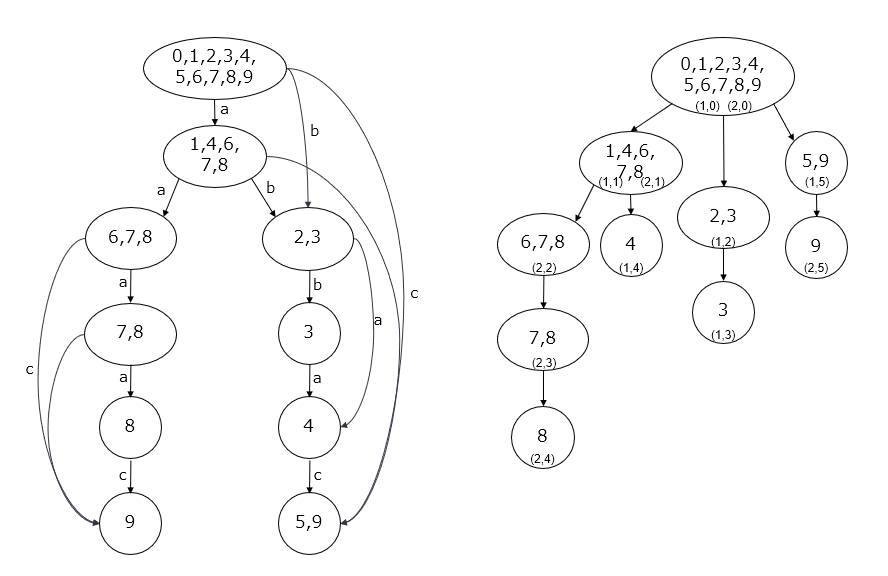
\includegraphics[width=15cm]{subcon.png}
    \caption{$D=\{"abcba", "abbac"\}$から構築した索引(左:ファクターオラクル、右:部分集合木)}
  \end{figure}


  \subsection{検索アルゴリズム}
  ここまでで、文字列集合に対するファクターオラクルを使用した索引は、文字列集合に対するファクターオラクル$M_{FO}$と部分集合木$T_W$の2つのデータ構造で構成されることが分かった。本節ではこの索引を使用した検索アルゴリズムを述べる。

  \begin{algorithm}
    \caption{$\textbf{Search}(P)$}
    \label{alg6}
    \begin{algorithmic}
      \State Input $P$
      \State $M_{FO}にPを入力$
      \State $f=\delta(s_0,P)とする$
      \If {$f \in F'$}
      \State $f \in Vを根とする部分木にある位置情報(i,j)を全て取り出す$
      \EndIf
      \State $各位置情報についてT_iのj文字目から先頭方向にPと比較し、一致したらRに位置情報を加える$
      \Return $R$
    \end{algorithmic}
  \end{algorithm}

  この検索アルゴリズムの実行時間は$\mathcal{O}(p \times |M_{FO}|)$である。
  また構築にも$|M_{FO}|^2$の時間がかかる。

  \chapter{提案手法}
  本章では、本研究の提案手法を解説する。

  \section{先行研究の問題点と改善案}
  文字列集合に対するファクターオラクルを用いた索引は、文字列集合から構築したトライ木の状態数を$n$、検索パターン長を$p$としたとき、構築に$\mathcal{O}(n^2)$、検索に$\mathcal{O}(p \times n)$の時間がかかることが分かった。

  本研究では、構築を$\mathcal{O}(n)$、検索を$\mathcal{O}(pの出現回数)$に改善する。

  方針としては、3章で述べた単一テキストに対して線形時間で構築と検索を行うことができるAllauzenの構築アルゴリズムとKatoの検索アルゴリズムを複数文字列に拡張することを考える。さらに、DFA最小化アルゴリズムを適用することでさらなる少サイズ化を試みる。

  提案アルゴリズムは3つの手順で構成される。
  \begin{enumerate}
    \item 入力の文字列集合からトライ木を構成する
    \item トライ木に拡張したAllauzenのアルゴリズムを適用し、文字列集合に対するファクターオラクルを構築する
    \item 文字列集合に対するファクターオラクルを最小化する
  \end{enumerate}

  \section{Allauzenのアルゴリズムの拡張}
  先述の通り、Allauzenのアルゴリズムは入力として単一テキスト$T$を入力とすることで$T$に対するファクターオラクルを構築しているため、入力を文字列集合に拡張する必要がある。そこで、前章の先行研究と同様に文字列集合から構築したトライ木を入力とすることでこれを解決する。

  拡張したAllauzenのアルゴリズムを以下に示す。

  \begin{algorithm}
    \caption{$\textbf{create\_oracle}(M)$}
    \label{alg7}
    \begin{algorithmic}[1]
      \State $Create\ Oracle(\epsilon)\ with:$
      \State $\ \ \ \ one\ single\ state\ 0$
      \State $\ \ \ \ S_\epsilon(0) \leftarrow -1$
      \For{\textbf{all}\ $q \in Q$}
        \For{\textbf{all}\ $\sigma \in \Sigma$}
          \State $i \leftarrow \delta(q, \sigma)$
          \State $Oracle \leftarrow add\_state(Oracle, q, \sigma, i)$
        \EndFor
      \EndFor
      \Return $Oracle$
    \end{algorithmic}
  \end{algorithm}
  
  関数add\_stateの定義は以下のようになっている。

  \begin{algorithm}
    \caption{$\textbf{add\_state}(Oracle, q, \sigma, i)$}
    \label{alg8}
    \begin{algorithmic}[1]
      \State $Create\ a\ new\ state\ i$
      \State $Create\ a\ new\ transition\ from\ q\ to\ i\ labbeled\ by\ \sigma$
      \State $k \leftarrow S(q)$
      \While{$k>-1\ and\ there\ is\ no\ transition\ from\ k\ by\ \sigma$}
      \State $Create\ a\ new\ transition\ from\ k\ to\ i\ by\ \sigma$
      \State $k \leftarrow S(k)$
      \EndWhile
      \If{$k=-1$}
      \State $s \leftarrow 0$
      \Else
      \State $s \leftarrow where\ leads\ the\ transition\ from\ k\ by\ \sigma.$
      \EndIf
      \State $S(i) \leftarrow s$
      \State \textbf{return} $Oracle$
    \end{algorithmic}
  \end{algorithm}

  具体例として、$p=$'abbbaab'をcreate\_oracleの実行例を以下に示す。
  \newpage

  \begin{figure}[htbp]
    \centering
    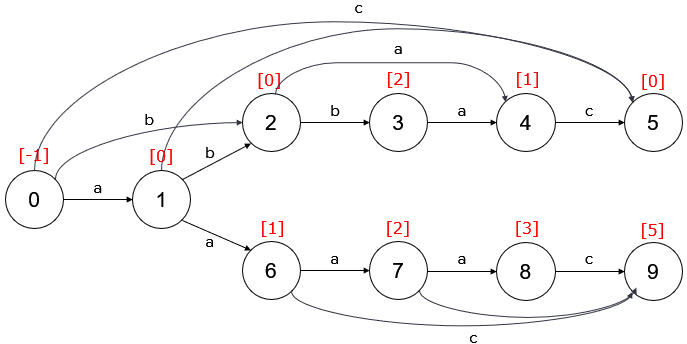
\includegraphics[width=15cm]{mfo.png}
    \caption{create\_oracleによるOracle('abbbaab')の構成例\ 各状態上の赤字はsupply functionを示す\ \cite{allauzen}より引用}
  \end{figure}

  \section{ファクターオラクルの最小化}
  本節では、ファクターオラクルの最小化について述べる。
 ファクターオラクルを最小化することによって、より索引の省サイズ化が見込める。

  オートマトンの状態数を$n$と置く。DFAの最小化には、一般的には$\mathcal{O}(n^2)$を要するが、非巡回型DFAから構成したファクターオラクルは常に非巡回型DFAであるため、ここでは$\mathcal{O}(n)$で動作する非巡回型DFAに対する最小化アルゴリズムを用いる。

  また、ファクターオラクルの最小化をより検索に支障が出ない範囲の内で効率的に行うため、最小化の際の等価性の検証には内部遷移のみを使用する。

  以下に非巡回型DFAを入力とする最小化アルゴリズムを示す。
  \begin{enumerate}
    \item 入力のDFAの状態のうち、遷移を持たない状態を統合する。
    \item 統合された状態に、同じラベルでの遷移を持つ状態を統合する。
    \item 統合が続く、もしくは初期状態に到達するまで2を繰り返す。
  \end{enumerate}

  また、統合された状態の情報は検索アルゴリズムで使用するため、保持しておく必要がある。

  \begin{figure}[htbp]
    \centering
    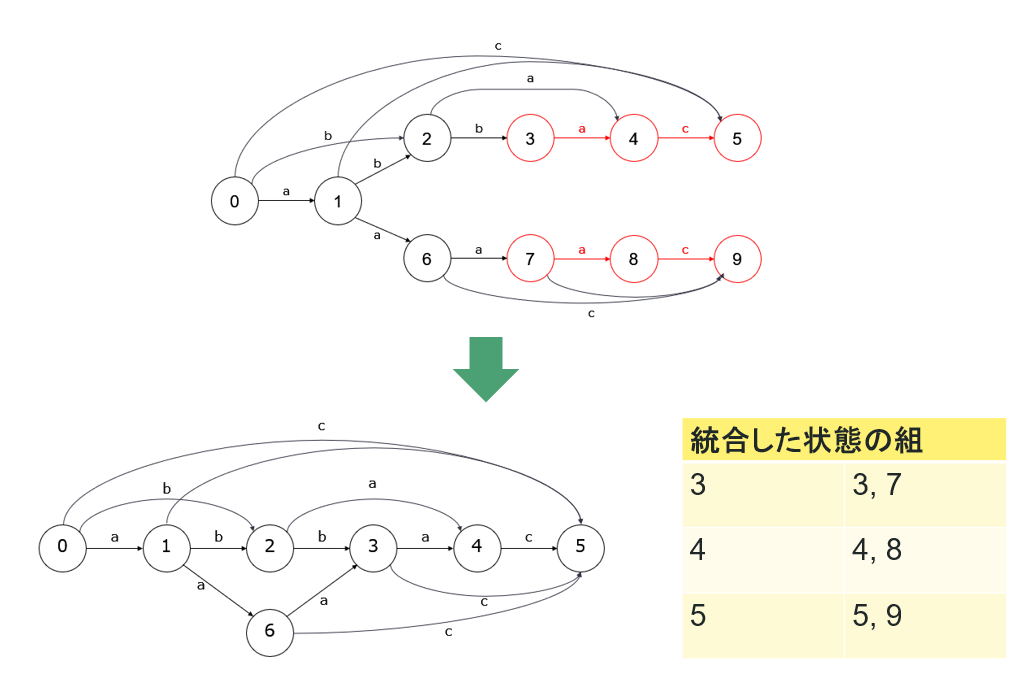
\includegraphics[width=15cm]{pair.png}

    \caption{ファクターオラクル最小化の例}
  \end{figure}
  
  \section{検索アルゴリズム}

  本章で解説した文字列集合に対するファクターオラクルの構築アルゴリズムは3章で解説したファクターオラクルのものと非常に似ており、検索アルゴリズムも同様である。

  変更点としては、最初の判定で最小化によって統合された状態全てに対して検証する必要がある点と、複数テキストを入力としているために、状態番号がそのまま出現位置を示さなくなった点がある。そのため本手法では、最小化によって統合された状態番号を保持する$pair$と各状態に対応する位置情報を保持する$endpos$という配列を定義している。
  
  本節では、アルゴリズムで使用する$SP_{-1}、S_{-1}, endpos$の実装方法について解説した後、検索アルゴリズムを示す。

  \subsection{検索アルゴリズムで使用するデータの表現}

  $SP_{-1}$を素直に実装すると、最悪の場合ファクターオラクルの状態数$n$の二乗の空間を使用する。

  これを解消するため、$SP_{-1}$をサフィックスリンクツリーのあるノードの子孫ノードの集合を保持するのではなく、子孫ノード集合の番号の最小値と最大値の組のみを保持するように変更することで、要素数$n$のタプルの配列として実装できる。(使用空間: $2 \times n$)
  
  しかし、子孫ノード集合を最小値と最大値をによって表現するためには、任意の集合が常に連番であるようなノードの集合である必要がある。Allauzenのアルゴリズムで構成されたサフィックスリンクツリーは常にそうなっているわけではないため、サフィックスリンクツリーを深さ優先探索で辿り、番号付けし直すことでこれを解決する。

  \begin{figure}[htbp]
    \centering
    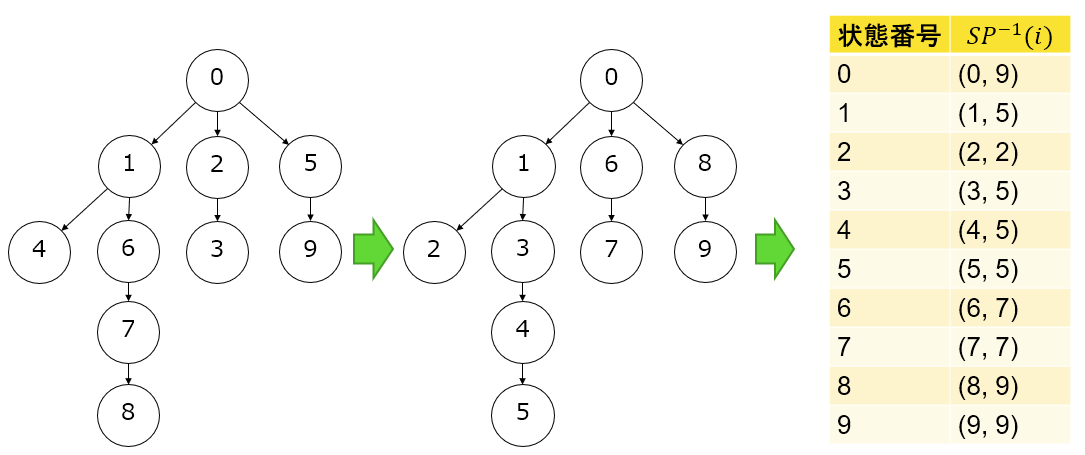
\includegraphics[width=15cm]{sp.png}

    \caption{$SP_{-1}の配列での実装$}
  \end{figure}
  \newpage

  また、$S_{-1}、endpos$の実装は以下のようになっている。

  \begin{figure}[htbp]
    \centering
    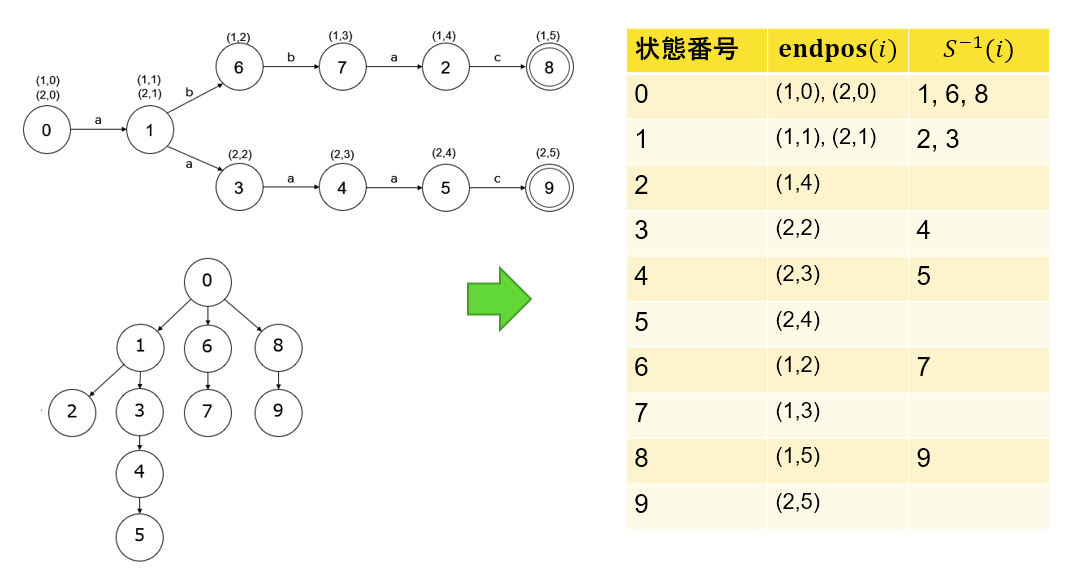
\includegraphics[width=15cm]{se.png}

    \caption{$S_{-1}とendposの配列での実装$}
  \end{figure}
  \newpage

  \subsection{提案アルゴリズム}
  ここでは、提案手法の検索アルゴリズムを示す。

  検索アルゴリズムは、
  \begin{enumerate}
    \item まず最初に入力のパターン$w$で$Oracle(p)$を遷移させ、受理した状態番号$\overline{w}$を得る。受理しなければ空集合を返す。
    \item その状態番号と統合された状態に対応するテキスト$p$の位置に$w$が出現していれば出現位置の集合$output$に$\overline{w}のendpos$を追加する。
    \item $Oracle(D)$があるパターン$w$を受理した場合の出現位置の候補は$\overline{w}$だけではなく、$SP(\overline{w})$の全てに及ぶ。よって、Algorithm\ 3の9行目からは、テキスト集合$D$の各$j \in S^{-1}(\overline{w})$の値に対して$w$が出現しているか判定している。もし出現していれば、$outputにSP^{-1}(j)の全てのendpos$を追加し、そうでなければ追加しない。
  \end{enumerate}

  \begin{algorithm}
    \caption{$\textbf{search}(Oracle(D), w)$}
    \label{alg9}
    \begin{algorithmic}[1]
      \If {$w\ recognized\ by\ Oracle(D)\ at state\ \overline{w}$}
        \State $x \leftarrow \overline{w}\ of\ Oracle(D)$
      \Else
      \ \Return $\emptyset \ \ \ \ \ \ \ \ \ \ \ \ \ \ \ \ \ /*\ empty\ set\ */$
      \EndIf
      \For {\textbf{all}\ $i \in pair(x)\ \ \ \ \ \ /*\ outer\ loop\ */$}
        \For {\textbf{all}\ $(s, t) \in endpos(i)$}
          \If {$D[s][(t-|w|+1)...t]=w$}
            \State $output(w)\leftarrow (s,t),\ break\ outer\ loop$
          \EndIf
        \EndFor
      \EndFor

      \For{$j \in S^{-1}(i)$}
        \For {\textbf{all}\ $(s, t) \in endpos(j)$}
          \If {$D[s][(t-|w|+1)...t]=w$}
            \For {$k \in SP_{-1}(j)$}
              \State $output(w)\leftarrow output(w) \cup endpos(j)$
            \EndFor
          \EndIf
        \EndFor
      \EndFor
      \Return {$output(w)$}
    \end{algorithmic}
  \end{algorithm}

  このアルゴリズムは、3章のKatoの検索アルゴリズムと同様に$\mathcal{O}(|S^{-1}(\overline{w}) \times w)$の実行時間を要す。$\mathcal{O}(|S^{-1}(i))|$は最悪で$\mathcal{O}(n)$になる。しかし、$Oracle(D)$のサフィックスリンクツリーのノード数が$n$であるため、ならし計算量では$\mathcal{O}(1)$となることがわかる。

  よってアルゴリズム全体でのならし計算量は$\mathcal{O}(max(w, output))$である。

%  \begin{figure}[htbp]
%    \centering
%
%    \caption{ファクターオラクルの検索の実行例}
%  \end{figure}

  \chapter{実験的評価}
  本章では、提案手法と部分集合構成法を用いた手法での構築と検索に要した時間を比較する。

  \section{実験結果}
  \begin{figure}[htbp]
    \centering

    \caption{実験結果}
  \end{figure}

  実験結果から、提案手法を用いた索引のほうが構築、検索の両方において効率的に行うことができるということが分かった。これは理論上も実行時間のオーダーから明らかであるため、納得の行く結果となった。

  \section{実験環境}
  実験に使用した環境を示す。

  \begin{description}
    \item[OS]\ \ \ \ \ \ \ \ \ \ \ \ CentOS 6.10
    \item[メモリ]\ \ \ \ \ \ 64GB
    \item[CPU]\ \ \ \ \ \ \ \ \ Intel Core i7-6850k\ (6\ core\ 3.6GHz)
    \item[テキスト]\ \ Enron\ mail\ dataset
  \end{description}

  \chapter{まとめ}

  本稿では文字列集合に対するファクターオラクルを用いたコンパクトな全文検索索引を提案した。

  コンパクトな全文検索索引を効率的に構築するため、Allauzenのアルゴリズムを拡張することで$\mathcal{O}(n)$の実行時間を得た。
  
  また、提案手法では内部遷移のみに注目したDFAの最小化を実行しているため、文字列集合に対して最も小さいオートマトンを構成できたと考えられる。

  今回の手法は、\cite{dawg-bit}と組み合わせることでより効率的に実装できることが考えられる。、



  \begin{thebibliography}{10}
    \bibitem{allauzen} C. Allauzen, M. Crochemore, M. Raffinot, "Factot Oracle: a new structure for pattern matching" Proc. Of SOSFSEM'99, LNCS, Vol.1725, p.295-310, 1999.
    \bibitem{kato} Ryoichi Kato, Osamu Watanabe, "Substring search and repeat search using factor oracles", Information Processing Letters, Vol.93, p269-274, 2005.
    \bibitem{ohi} 大井恒平, "ファクターオラクルの拡張とその応用に関する研究", 2019.
    \bibitem{dawg} A. Blumer and J. Blumer and D. Haussler, ”The smallest automaton recognizing the subwords of a text.” ,Theoretical Computer Science, Vol.40, p31-55, 1985.
    \bibitem{dawg-bit} Miroslav Balik, "DAWG versus Suffix Array", CIAA'02: Proceedings of the 7th international conference on Implementation and application of automata, p.233-238, 2002.
  \end{thebibliography}

  \section*{謝辞}
本研究を行うにあたって、指導教員である山本博章先生には熱心なご指導ご鞭撻を賜り、ありがとうございました。また、藤原洋志先生には、ゼミ等で数々のご指摘やご助言を賜りました。ここに感謝の意を表します。
\end{document}

